% Created with jtex v.0.1.12
%% 
%% Copyright 2007-2020 Elsevier Ltd
%% 
%% This file is part of the 'Elsarticle Bundle'.
%% ---------------------------------------------
%% 
%% It may be distributed under the conditions of the LaTeX Project Public
%% License, either version 1.2 of this license or (at your option) any
%% later version.  The latest version of this license is in
%%    http://www.latex-project.org/lppl.txt
%% and version 1.2 or later is part of all distributions of LaTeX
%% version 1999/12/01 or later.
%% 
%% The list of all files belonging to the 'Elsarticle Bundle' is
%% given in the file `manifest.txt'.
%% 
%% Template article for Elsevier's document class `elsarticle'
%% with harvard style bibliographic references

\documentclass[review,authoryear,12pt]{elsarticle}

%% The lineno packages adds line numbers. Start line numbering with
%% \begin{linenumbers}, end it with \end{linenumbers}. Or switch it on
%% for the whole article with \linenumbers.
%% \usepackage{lineno}

% Packages
\usepackage{amsmath}

% You should have an imports section
%%%%%%%%%%%%%%%%%%%%%%%%%%%%%%%%%%%%%%%%%%%%%%%%%%
%%%%%%%%%%%%%%%%%%%%  imports  %%%%%%%%%%%%%%%%%%%
\usepackage{framed}
\usepackage{graphicx}
\usepackage{hyperref}
\usepackage{natbib}
\usepackage{url}
%%%%%%%%%%%%%%%%%%%%%%%%%%%%%%%%%%%%%%%%%%%%%%%%%%

% Journal name
\journal{Nuclear Physics B}

\begin{document}

% Frontmatter
\begin{frontmatter}

% Title
\title{Pixels and Their Neighbours}

% Authors and Affiliations
\author[1]{Rowan Cockett}\author[1]{Lindsey Heagy}\author[1]{Douglas Oldenburg}
\affiliation[1]{University of British Columbia}

% Abstract
\begin{abstract}
In this tutorial we take you on the journey from continuous equations to their discrete matrix representations using the finite volume method for the Direct Current (DC) resistivity problem. These techniques are widely applicable across geophysical simulation types and have their parallels in finite element and finite difference. We show derivations visually, as you would on a whiteboard, and have provided an accompanying notebook to explore the numerical results using \href{http://simpeg.xyz/}{SimPEG}.
\end{abstract}

% Graphical abstract
\begin{graphicalabstract}
\end{graphicalabstract}

% Highlights

% Keywords
\begin{keyword}
Finite volume \sep Direct current \sep Resistivity \sep DC equations
\end{keyword}

\end{frontmatter}

%% \linenumbers

\begin{framed}
\textbf{Important}\\
This article was originally published in the Leading Edge (\cite{Cockett_2016}) and is licensed under \href{https://creativecommons.org/licenses/by-sa/3.0/}{CC-BY-SA-3.0}.
\end{framed}

\section{DC Resistivity}\label{DC Resistivity}

DC resistivity surveys obtain information about subsurface electrical conductivity, $\sigma$. This physical property is often diagnostic in mineral exploration, geotechnical, environmental and hydrogeologic problems, where the target of interest has a significant electrical conductivity contrast from the background. In a DC resistivity survey, steady state currents are set up in the subsurface by injecting current through a positive electrode and completing the circuit with a return electrode (Figure~\ref{dc-setup}).

\begin{figure}[!htbp]
\centering
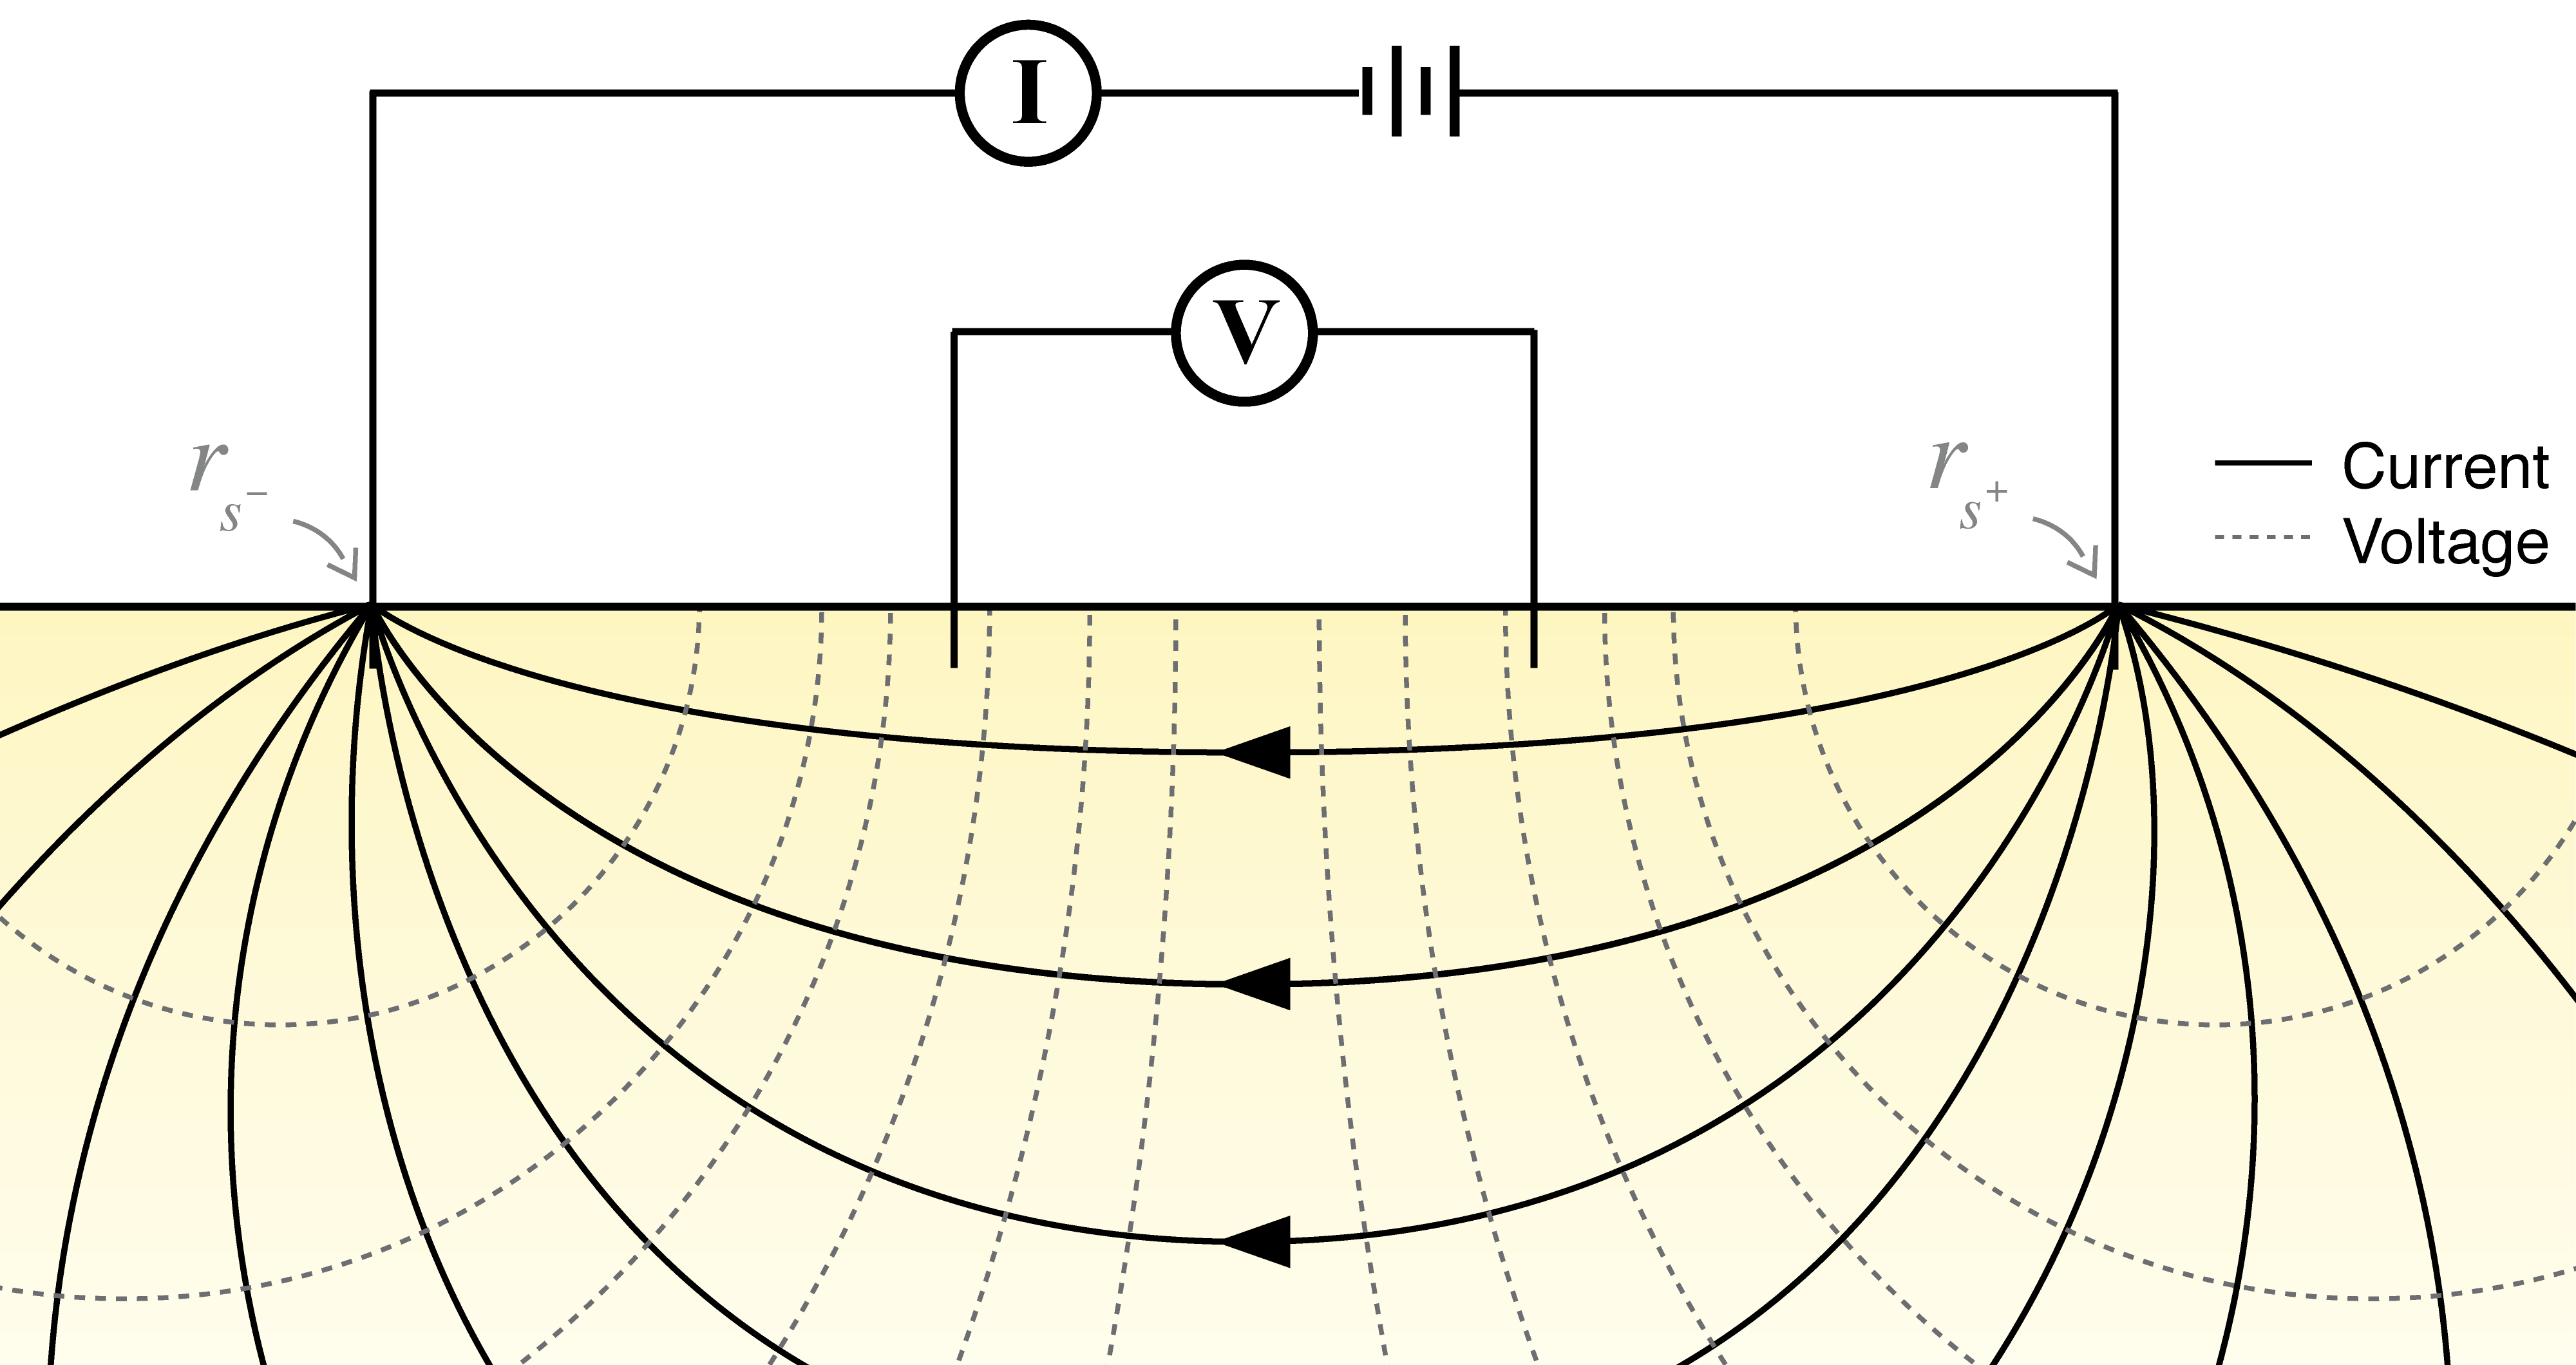
\includegraphics[width=0.9\linewidth]{files/dc-setup-652f2205515a8a5b83384bc6c2553b21.png}
\caption{Setup of a DC resistivity survey.}
\label{dc-setup}
\end{figure}

The equations for DC resistivity are derived in (Figure~\ref{dc-eqns}). Conservation of charge (which can be derived by taking the divergence of Ampere's law at steady state) connects the divergence of the current density everywhere in space to the source term which consists of two point sources, one positive and one negative.

The flow of current sets up electric fields according to Ohm's law, which relates current density to electric fields through the electrical conductivity. From Faraday's law for steady state fields, we can describe the electric field in terms of a scalar potential, $\phi$, which we sample at potential electrodes to obtain data in the form of potential differences.

\begin{figure}[!htbp]
\centering
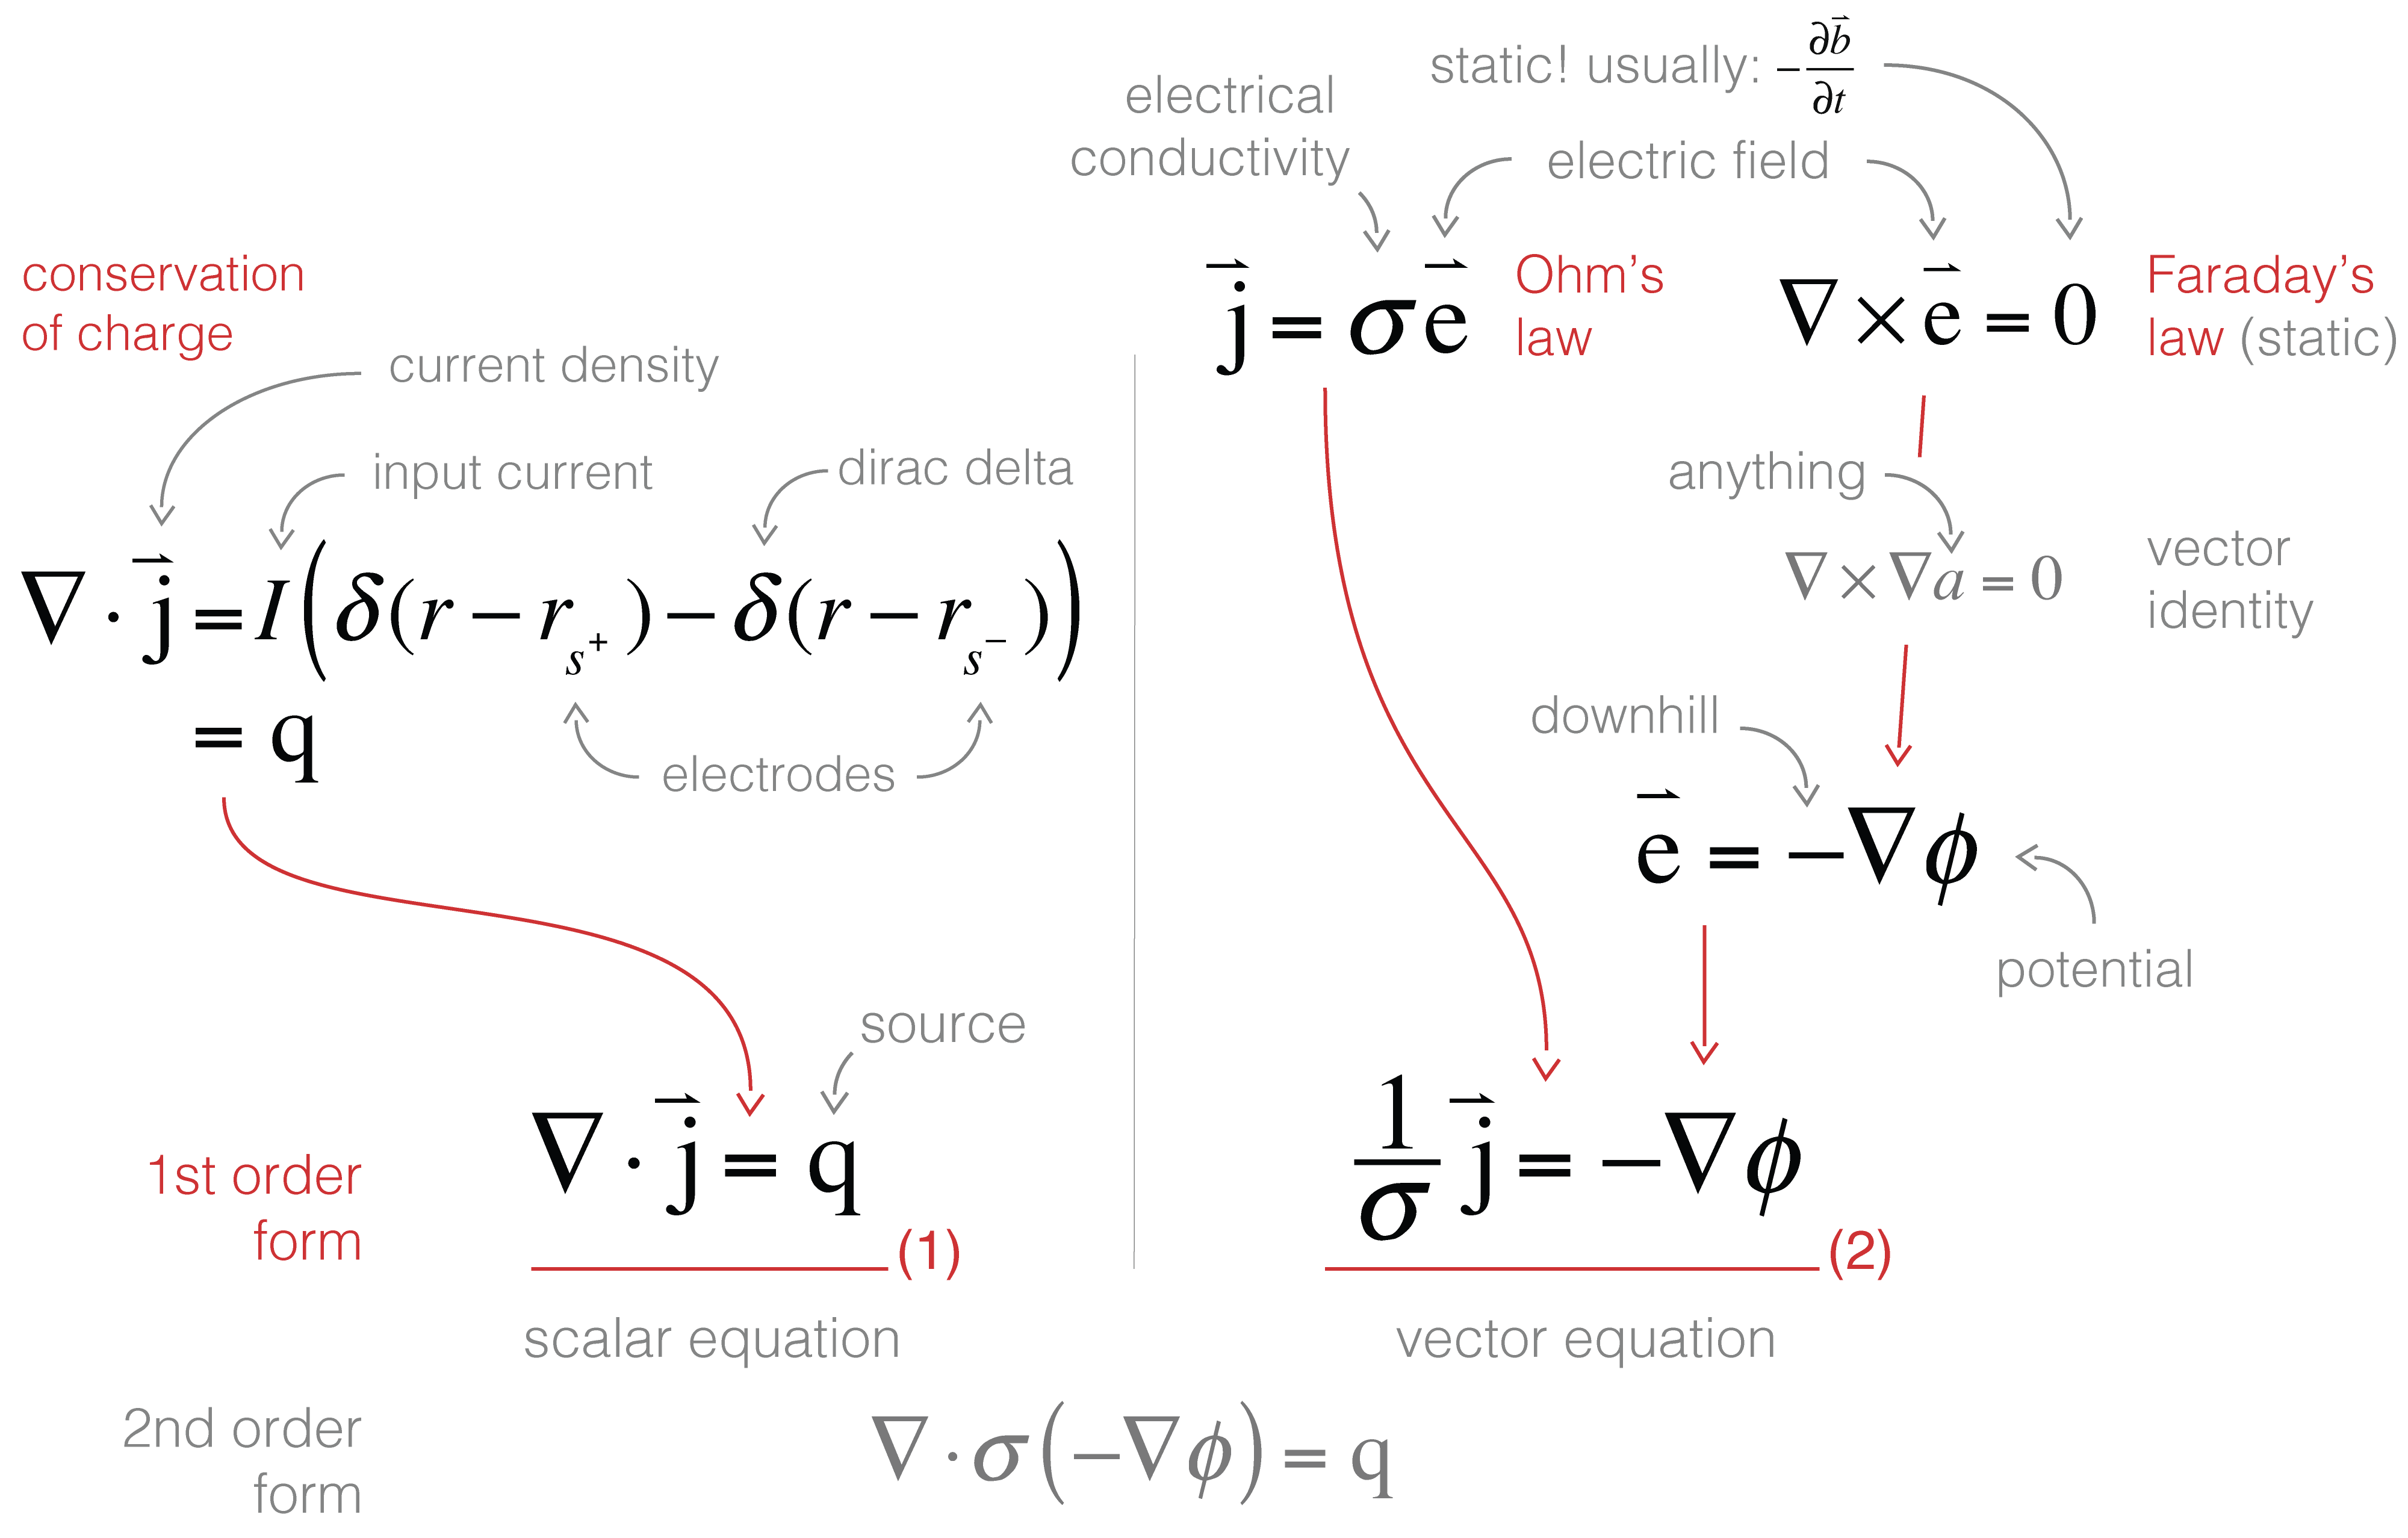
\includegraphics[width=0.7\linewidth]{files/dc-eqns-24aa019a0163d3158b1e938ceea962a6.png}
\caption{Derivation of the DC resistivity equations.}
\label{dc-eqns}
\end{figure}

To set up a solvable system of equations, we need the same number of unknowns as equations, in this case two unknowns (one scalar, $\phi$, and one vector $\vec{j}$) and two first-order equations (one scalar, one vector).

In this tutorial, we walk through setting up these first order equations in finite volume in three steps: (1) defining where the variables live on the mesh; (2) looking at a single cell to define the discrete divergence and the weak formulation; and (3) moving from a cell based view to the entire mesh to construct and solve the resulting matrix system. The notebooks included with this tutorial leverage the \href{http://simpeg.xyz/}{SimPEG} package, which extends the methods discussed here to various mesh types.

\section{Where do things live?}\label{Where do things live?}

To bring our continuous equations into the computer, we need to discretize the earth and represent it using a finite(!) set of numbers. In this tutorial we will explain the discretization in 2D and generalize to 3D in the notebooks. A 2D (or 3D!) mesh is used to divide up space, and we can represent functions (fields, parameters, etc.) on this mesh at a few discrete places: the nodes, edges, faces, or cell centers. For consistency between 2D and 3D we refer to faces having area and cells having volume, regardless of their dimensionality. Nodes and cell centers naturally hold scalar quantities while edges and faces have implied directionality and therefore naturally describe vectors. The conductivity, $\sigma$, changes as a function of space, and is likely to have discontinuities (e.g. if we cross a geologic boundary). As such, we will represent the conductivity as a constant over each cell, and discretize it at the center of the cell. The electrical current density, $\vec{j}$, will be continuous across conductivity interfaces, and therefore, we will represent it on the faces of each cell. Remember that $\vec{j}$ is a vector; the direction of it is implied by the mesh definition (i.e. in $x$, $y$ or $z$), so we can store the array $\mathbf{j}$ as \textit{scalars} that live on the face and inherit the face's normal. When $\vec{j}$ is defined on the faces of a cell the potential, $\phi$, will be put on the cell centers (since $\vec{j}$ is related to $\phi$ through spatial derivatives, it allows us to approximate centered derivatives leading to a staggered, second-order discretization). Once we have the functions placed on our mesh, we look at a single cell to discretize each first order equation. For simplicity in this tutorial we will choose to have all of the faces of our mesh be aligned with our spatial axes ($x$, $y$ or $z$), the extension to curvilinear meshes will be presented in the supporting notebooks.

\begin{figure}[!htbp]
\centering
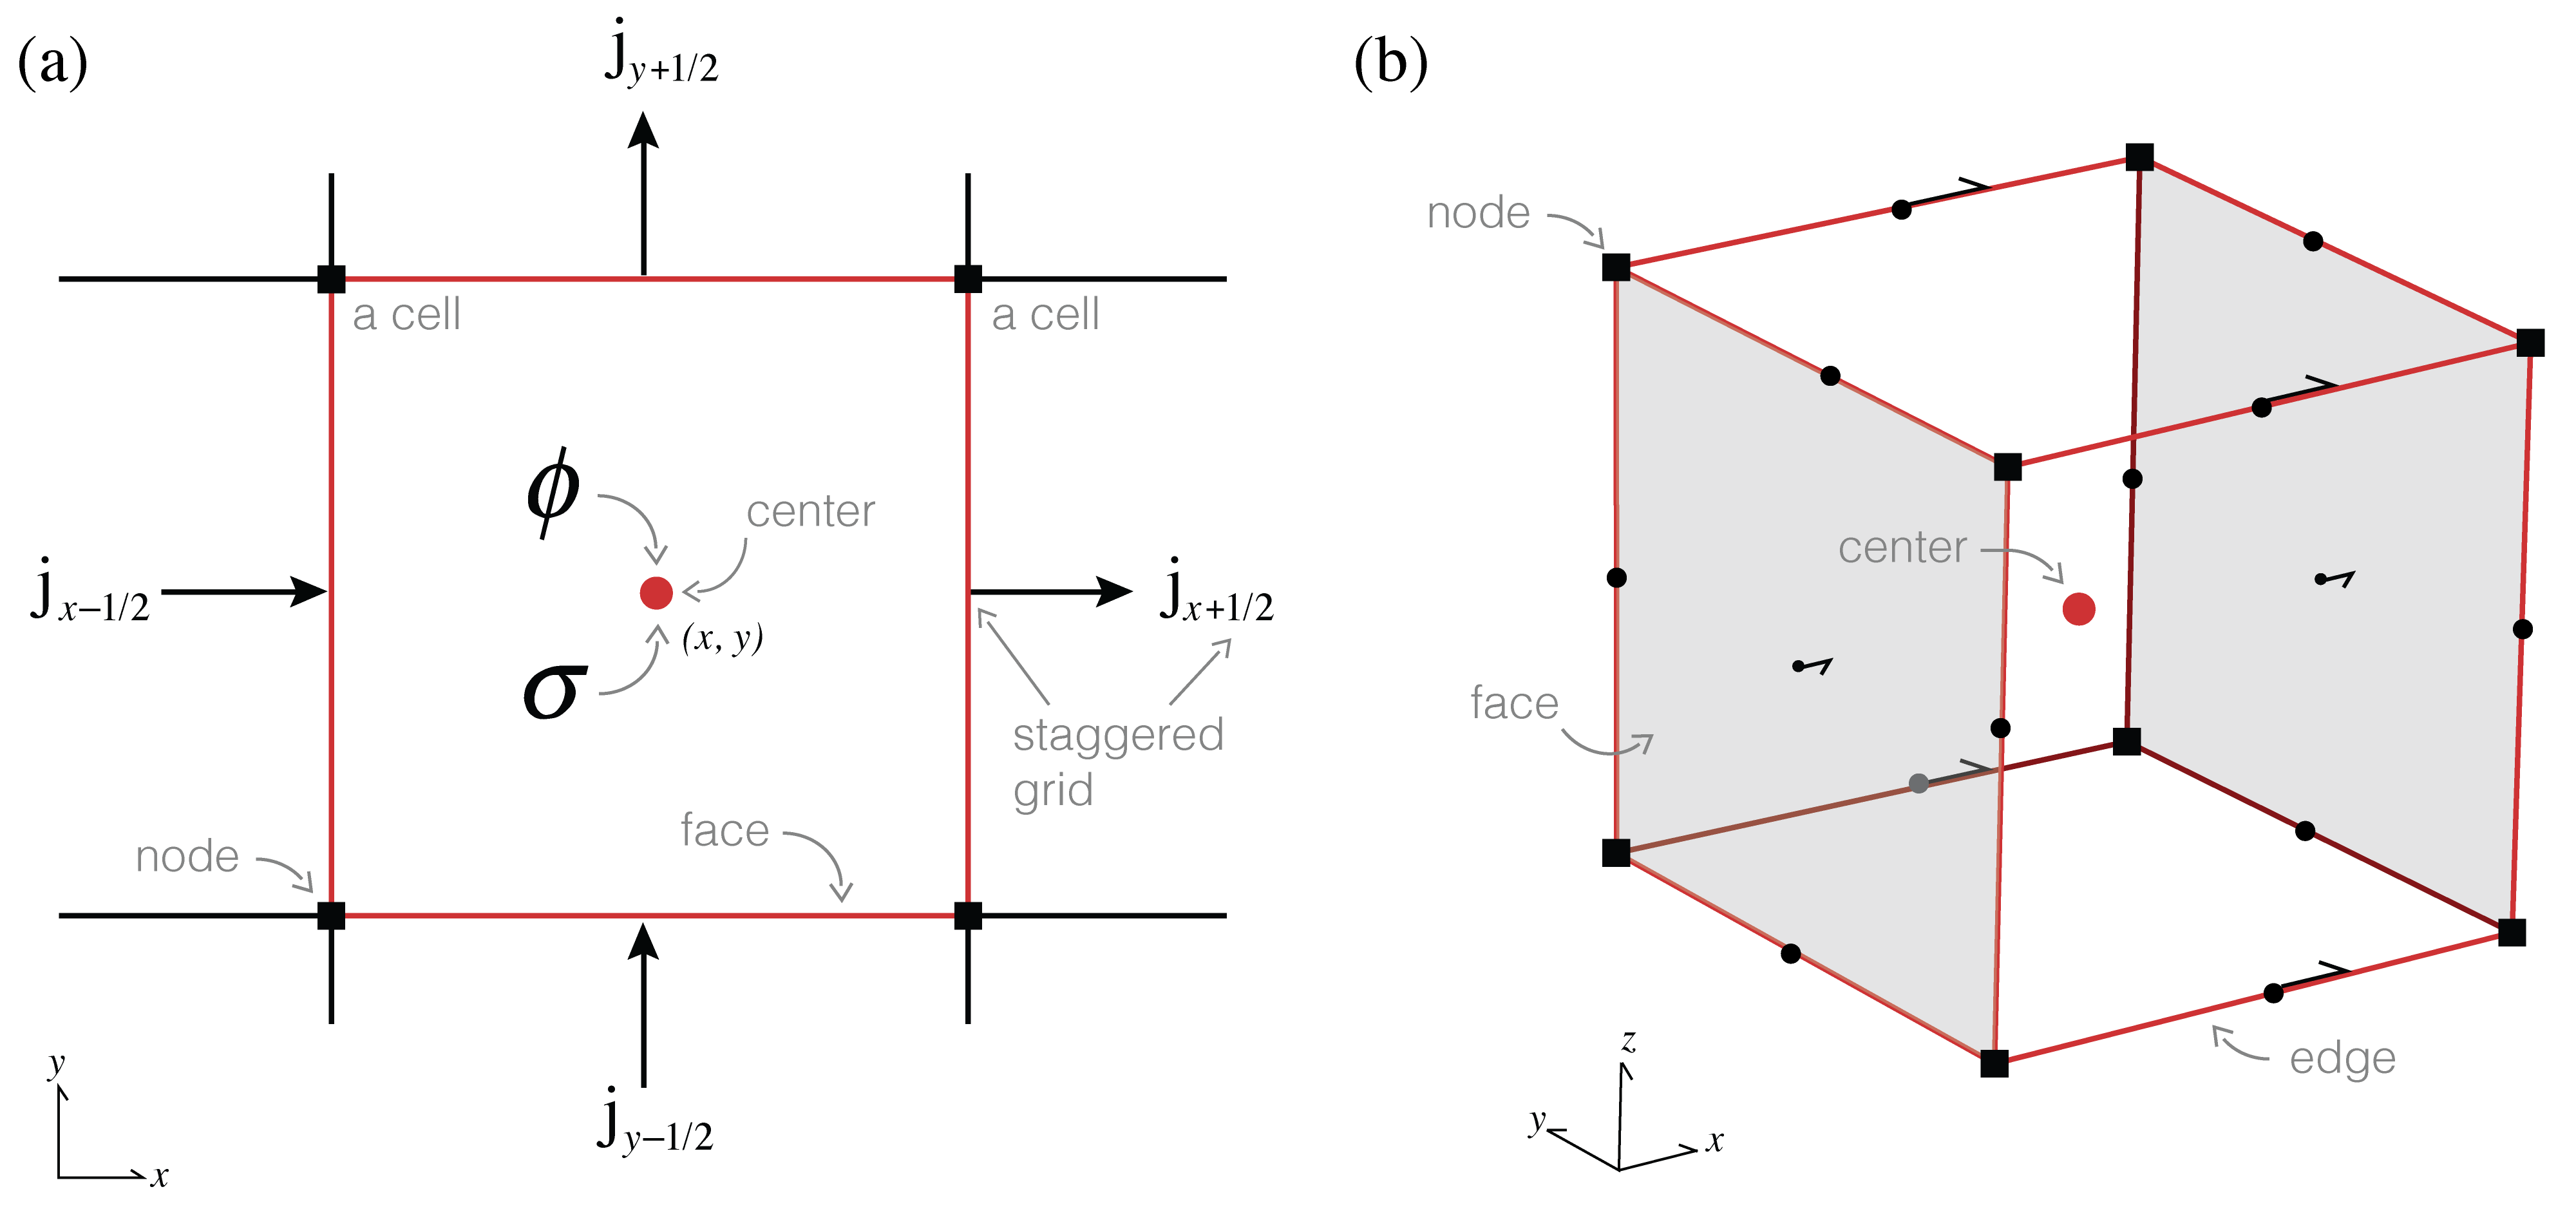
\includegraphics[width=1\linewidth]{files/mesh-5a1ece0e8f4ddb6e3e03e641b4236ca1.png}
\caption{Anatomy of a finite volume cell.}
\label{fig-mesh}
\end{figure}

\section{One cell at a time}\label{One cell at a time}

To discretize the first order differential equations we consider a single cell in the mesh and we will work through the discrete description of equations (1) and (2) over that cell.

\subsection{(1) In and out}\label{(1) In and out}

\begin{figure}[!htbp]
\centering
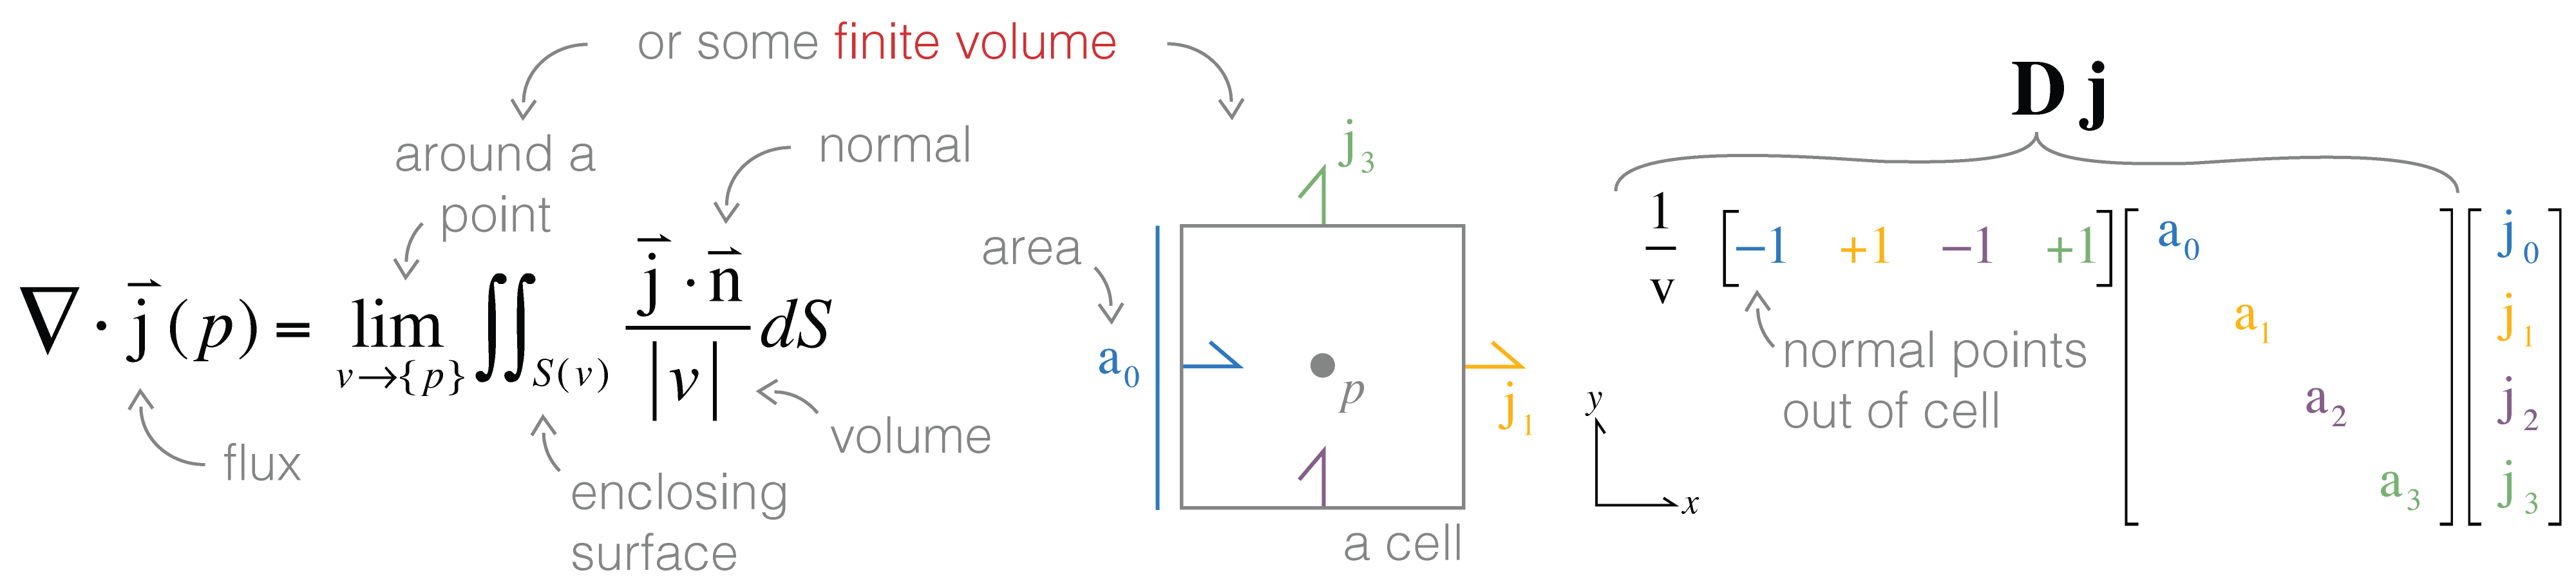
\includegraphics[width=0.9\linewidth]{files/divergence-aaa3fd78a0b3ca2af36eb8246f8ff063.png}
\caption{Geometrical definition of the divergence and the discretization.}
\label{fig-div}
\end{figure}

So we have half of the equation discretized - the left hand side. Now we need to take care of the source: it contains two dirac delta functions - these are infinite at their origins, $r_{s^+}$ and $r_{s^ -}$. However, the volume integral of a delta function \textit{is} well defined: it is \textit{unity} if the volume contains the origin of the delta function otherwise it is \textit{zero}.

As such, we can integrate both sides of the equation over the volume enclosed by the cell. Since $\mathbf{D}\mathbf{j}$ is constant over the cell, the integral is simply a multiplication by the volume of the cell $\text{v} \mathbf{D} \mathbf{j}$. The integral of the source is zero unless one of the source electrodes is located inside the cell, in which case it is $q = \pm I$. Now we have a discrete description of equation 1 over a single cell:

\begin{equation}
\label{eq:div}
\text{v} \mathbf{D}\mathbf{j} = q
\end{equation}

\subsection{(2) Scalar equations only, please}\label{(2) Scalar equations only, please}

Equation (\ref{eq:div}) is a vector equation, so really it is two or three equations involving multiple components of $\vec{j}$. We want to work with a single scalar equation, allow for anisotropic physical properties, and potentially work with non-axis-aligned meshes - how do we do this?! We can use the \textbf{weak formulation} where we take the inner product ($\int \vec{a} \cdot \vec{b} dv$) of the equation with a generic face function, $\vec{f}$. This reduces requirements of differentiability on the original equation and also allows us to consider tensor anisotropy or curvilinear meshes .

In Figure~\ref{fig-weak-formulation}, we visually walk through the discretization of equation (b). On the left hand side, a dot product requires a \textit{single} cartesian vector, $\mathbf{j_x, j_y}$. However, we have a $j$ defined on each face (2 $j_x$ and 2 $j_y$ in 2D!). There are many different ways to evaluate this inner product: we could approximate the integral using trapezoidal, midpoint or higher order approximations. A simple method is to break the integral into four sections (or 8 in 3D) and apply the midpoint rule for each section using the closest $\mathbf{j}$ components to compose a cartesian vector. A $\mathbf{P}_i$ matrix (size $2 \times 4$) is used to pick out the appropriate faces and compose the corresponding vector (these matrices are shown with colors corresponding to the appropriate face in the figure). On the right hand side, we use a vector identity to integrate by parts. The second term will cancel over the entire mesh (as the normals of adjacent cell faces point in opposite directions) and $\phi$ on mesh boundary faces are zero by the Dirichlet boundary condition. This leaves us with the divergence, which we already know how to do!

\begin{figure}[!htbp]
\centering
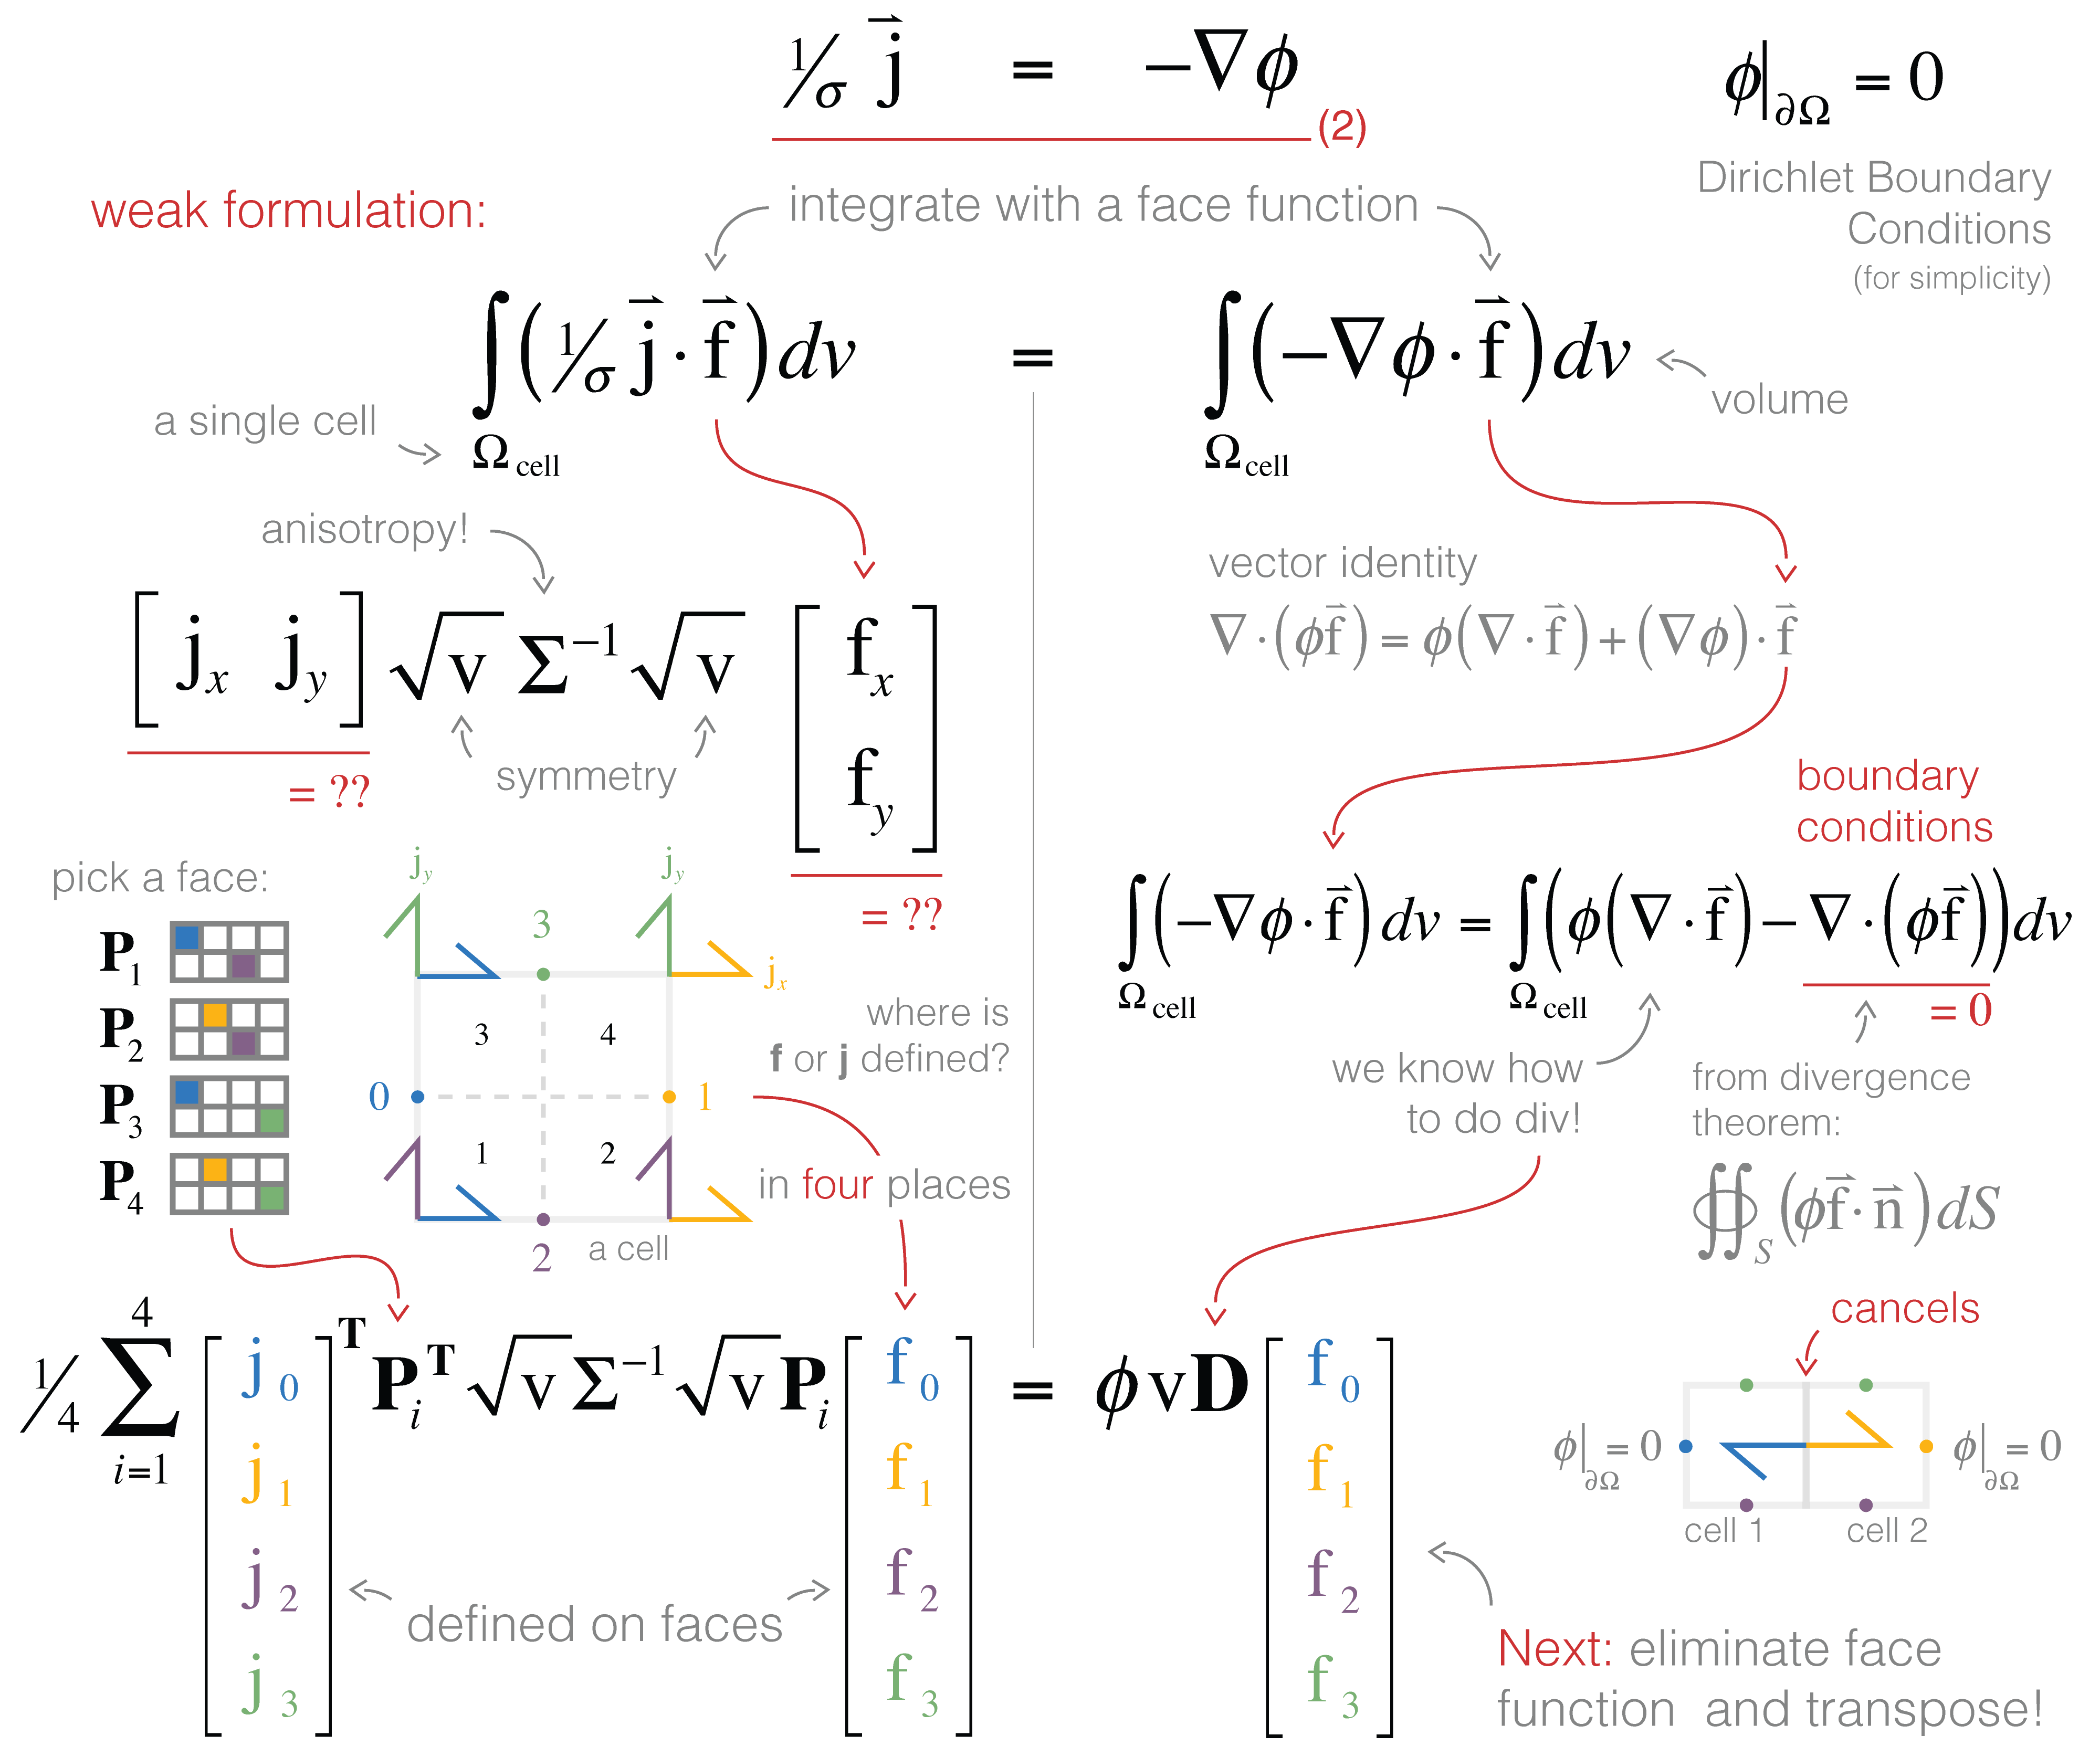
\includegraphics[width=1\linewidth]{files/weak-formulation-6a8027bb5c95916898575b76c126ffce.png}
\caption{Discretization using the weak formulation and inner products.}
\label{fig-weak-formulation}
\end{figure}

The final step is to recognize that, now discretized, we can cancel the general face function $\mathbf{f}$ and transpose the result (for convention's sake):

\begin{equation}
\frac{1}{4} \sum_{i=1}^4 \mathbf{P}_i^\top \sqrt{v} \mathbf{\Sigma}^{-1} \sqrt{v} \mathbf{P}_i \mathbf{j} = \mathbf{D}^\top v \phi
\end{equation}

\section{All together now}\label{All together now}

We have now discretized the two first order equations over a single cell. What is left is to assemble and solve the DC system over the entire mesh. To implement the divergence on the full mesh, the stencil of $\pm$1's must index into $\mathbf{j}$ on the entire mesh (instead of four elements). Although this can be done in a \texttt{for-loop}, it is conceptually, and often computationally, easier to create this stencil using nested Kronecker Products (see notebook). The volume and area terms in the divergence get expanded to diagonal matrices, and we multiply them together to get the discrete divergence operator. The discretization of the \textit{face} inner product can be abstracted to a function, $\mathbf{M}_f(\sigma^{ -1})$, that completes the inner product on the entire mesh at once. The main difference when implementing this is the $\mathbf{P}$ matrices, which must index into the entire mesh. With the necessary operators defined for both equations on the entire mesh, we are left with two discrete equations:

\begin{equation}
\text{diag}(\mathbf{v}) \mathbf{D}\mathbf{j} = \mathbf{q}
\end{equation}

\begin{equation}
\mathbf{M}_f(\sigma^{-1}) \mathbf{j} = \mathbf{D}^\top \text{diag}(\mathbf{v})\phi
\end{equation}

Note that now all variables are defined over the entire mesh. We could solve this coupled system or we could eliminate $\mathbf{j}$ and solve for $\phi$ directly (a smaller, second-order system).

\begin{equation}
\text{diag}({\mathbf{v}}) \mathbf{D}\mathbf{M}_f(\sigma^{-1})^{-1}\mathbf{D}^\top\text{diag}({\mathbf{v}})\phi = \mathbf{q}
\end{equation}

By solving this system matrix, we obtain a solution for the electric potential $\phi$ everywhere in the domain. Creating predicted data from this requires an interpolation to the electrode locations and subtraction to obtain potential differences!

\begin{figure}[!htbp]
\centering
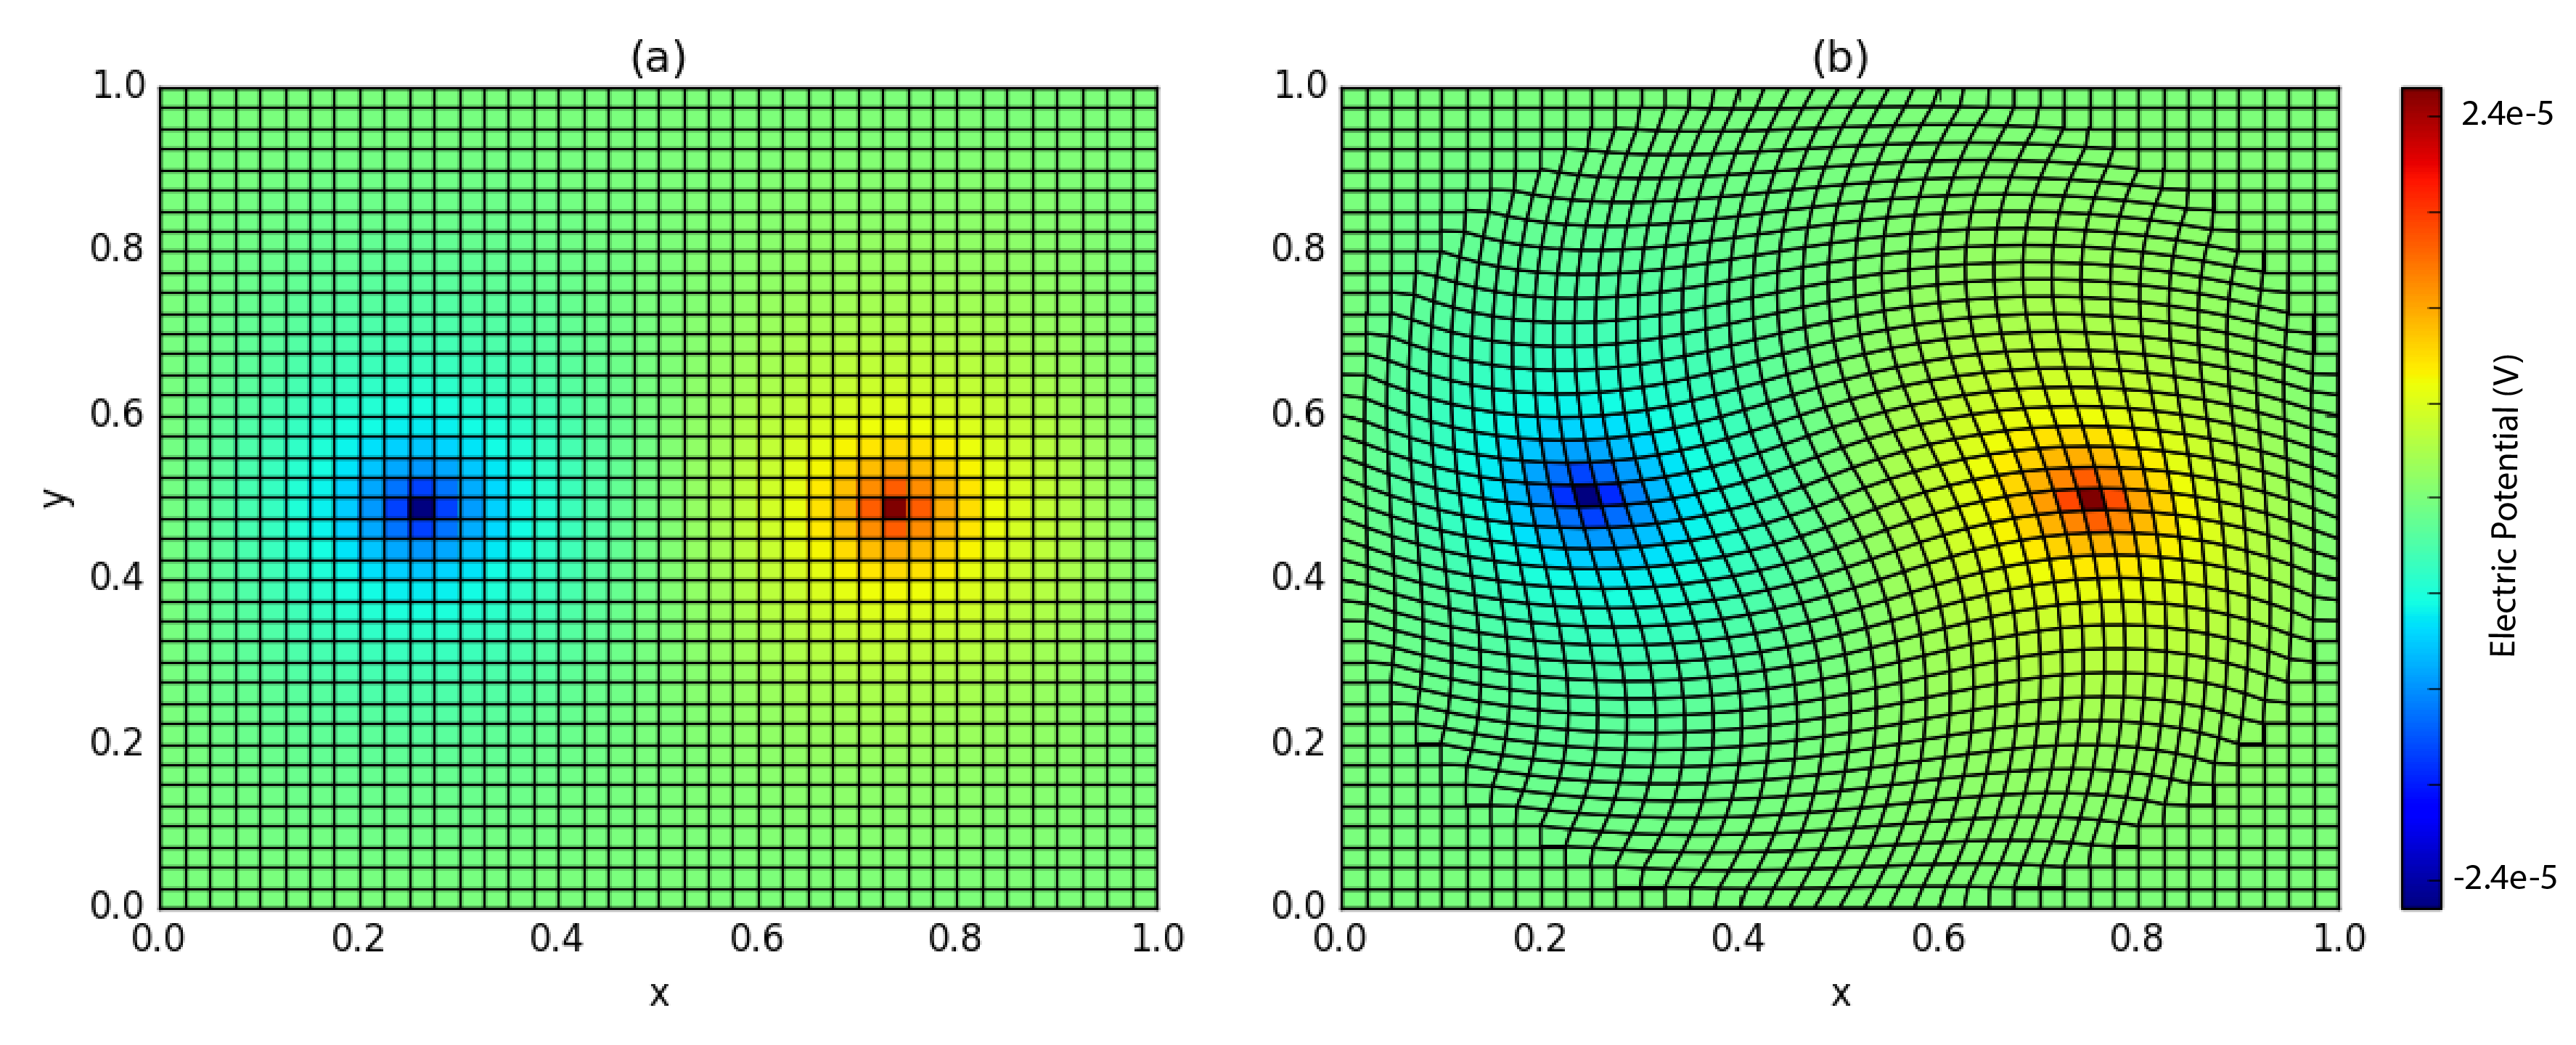
\includegraphics[width=1\linewidth]{files/dc-results-2a6cca42c68b08e6bdd9a053a98e9a28.png}
\caption{Electric potential on (a) tensor and (b) curvilinear meshes.}
\label{fig-results}
\end{figure}

Moving from continuous equations to their discrete analogues is fundamental in geophysical simulations. In this tutorial, we have started from a continuous description of the governing equations for the DC resistivity problem, selected locations on the mesh to discretize the continuous functions, constructed differential operators by considering one cell at a time, assembled and solved the discrete DC equations. Composing the finite volume system in this way allows us to move to different meshes and incorporate various types of boundary conditions that are often necessary when solving these equations in practice.

% Availability
\section*{Data Availability Statement}
Associated notebooks are available on \href{https://github.com/simpeg/tle-finitevolume}{GitHub} and can be run online with \href{http://mybinder.org/repo/simpeg/tle-finitevolume}{MyBinder}.


% Appendix
All article content, except where otherwise noted (including republished material), is licensed under a Creative Commons Attribution 3.0 Unported License (CC BY-SA). See \href{https://creativecommons.org/licenses/by-sa/3.0/}{https://creativecommons.org/licenses/by-sa/3.0/}. Distribution or reproduction of this work in whole or in part commercially or noncommercially requires full attribution of the \cite{Cockett_2016}, including its digital object identifier (DOI). Derivatives of this work must carry the same license. All rights reserved.

% Bibliography
\bibliographystyle{elsarticle-harv}
\bibliography{main.bib}

\end{document}
